\documentclass[conference]{IEEEtran}
\usepackage{graphicx}
\usepackage{algorithm}
\usepackage{algorithmic}

\makeatletter
\def\BState{\State\hskip-\ALG@thistlm}
\makeatother


\begin{document}
\title{Assignment 6 - Sort a given array by finding the max and min element using divide and conquer approach.}

\author{\IEEEauthorblockN{Parag Parihar}
\IEEEauthorblockA{Roll No:- IIT2016095\\
iit2016095@iiita.ac.in}
\and
\IEEEauthorblockN{Rakshit Sai}
\IEEEauthorblockA{Roll No:- IIT2016126\\
iit2016126@iiita.ac.in}
\and
\IEEEauthorblockN{Adarsh Agrawal}
\IEEEauthorblockA{Roll No:- IIT2016516\\
iit2016516@iiita.ac.in}
\and
\IEEEauthorblockN{Nilotpal Pramanik}
\IEEEauthorblockA{Roll No:- IRM2016501\\
irm2016501@iiita.ac.in}
\thanks{Manuscript received February 2, 2018.}}

\markboth{Assignment-1, IDAA432C; B.Tech.(IT)}
{Shell \MakeLowercase{\textit{et al.}}: Bare Demo of IEEEtran.cls for Journals}

\maketitle

\IEEEpeerreviewmaketitle
\begin{abstract}
Sort a given array by continuously tracking the max and min elements at every recursive step and placing the max and min elements at the correct position. find the max and min element using divide and conquer approach. 
\end{abstract}

\section{\textbf{Introduction and Literature Survey}}

The given problem is on divide and conquer. A typical Divide and Conquer algorithm solves a problem using following three steps.

1. Divide: Break the given problem into subproblems of same type.
2. Conquer: Recursively solve these subproblems
3. Combine: Appropriately combine the answers


The given problem for us is to sort a given array by continuously tracking the maximum and minimum elements at every recursive step and placing the maximum and minimum elements at the correct position. We need to find the maximum and minimum elements by using the divide and conquer approach. It basically means that we need to divide the array into two parts and then keep on solving the same way in subsequent steps and finally combine the array to arrive with the sorted array.  


The report contains :-\\
2. Algorithm Design\\
3. Analysis and Discussion\\
4. Experimental Analysis\\
5. Conclusion\\

\section{\textbf{Algorithm Design}}  
To implement this algorithm, it is our convention that we are sorting the array in \textbf{ascending order} through \textbf{divide and conquer approach}.So, now we have to scan an array of integers through taking the length of the array which are the inputs for this problem.After that we have to check weather the array is in ascending order or not.Thats why we will traverse the array up to half of its length and check weather the return value of the function \textbf{check} is 1 or not.For this function we are sending the constructed array according the current minimum and maximum index in each iteration of the loop.\\

\textbf{"check" Function:} Basically in this function we are checking weather the array is in ascending order or not.As the attributes we are taking the \textbf{array} itself along with the \textbf{start}: the starting index and \textbf{end}: the last index of the array.Then we are initializing a \textbf{flag} variable to 1,indicating the array is in ascending order.After that we are traversing the whole array from the starting index and check weather the current element is lesser than the previous one or not.If true then assign 0 at flag and break the loop.And from the function we are returning the value of flag.\\

Now if the return value of \textbf{check} is 1 then the input array is already sorted in ascending order and we have just to print that array accordingly.\\

Otherwise we have to store the return value of the \textbf{getMinMax} function in mx,the \textbf{struct pair}.\\

 
 \textbf{"struct pair" Structure:} This structure only contains the \textbf{min} and \textbf{max} to integers.\\

\textbf{"getMinMax" Function:} As the attributes it takes the \textbf{array}, \textbf{low}: the starting index and \textbf{high}: the last index of the array.As well as the return type of this function is \textbf{struct pair}.In the function we are defining the \textbf{minmax},\textbf{mml}(: struct pair for the left portion of the array),\textbf{mmr}(: struct pair for the right portion of the array) variables as the struct pair and \textbf{mid} variable as the integer data type.If the array consists only one element the the value of \textbf{low} and \textbf{high} will be equal and satisfying that condition the value of \textbf{low} will be assigned to \textbf{minmax.max} and \textbf{minmax.min} both.And return the \textbf{minmax}. If the array consists only two elements then we have only to check the value of \textbf{high} is just next to the value of \textbf{low} or not.If true then simply we have to determine the value at the \textbf{low}th index of the array is greater than the value at the \textbf{high}th index of the array and then we will assign the value of \textbf{low} to \textbf{minmax.max} and the value of \textbf{high} to \textbf{minmax.min}.Otherwise we have to assign the value of \textbf{high} to \textbf{minmax.max} and the value of \textbf{low} to \textbf{minmax.min} accordingly.
When the array consists more than two elements then we are assigning the value of (low + high)/2 in \textbf{mid} and through recursive way storing the value getMinMax(arr, low, mid) and getMinMax(arr, mid+1, high) in \textbf{mml} and \textbf{mmr} respectively.Basically here we are dividing the whole array with respect to the middle index of the array \textbf{mid} in \textbf{left} and \textbf{right}.Now we are comparing the maximum values and minimum values of the two partitions and finally determining the highest and lowest value among them and assigning their values in \textbf{minmax.max} and \textbf{minmax.min} respectively.And returning the \textbf{minmax} from this function which is containing the minimum and maximum indexes of the particular constructed array.\\

Now print the \textbf{minimum}: the element stored in \textbf{mx.min}th index of the array,\textbf{maximum}: the element stored in \textbf{mx.max}th index of the array followed by the range through printing the values of \textbf{0+i} and \textbf{n-1-i}.Now we have just to assign the minimum element of that particular constructed array in the lowest index and accordingly the maximum element in the highest index through swapping the values in that array.We have to follow this procedure in each iteration of the for loop traversing for the half of the length of the input array.And finally we are printing the sorted array in ascending order, according to our convention.\\

 

\begin{algorithm}[H]
\caption{getMinMax function}
\end{algorithm}
\begin{algorithmic}[1]
\STATE \textbf{INPUT: arr, start, end}
\STATE \textbf{OUTPUT: position of minimum and maximum element}
\STATE \textit{\textbf{Struct pair} minmax, mml, mmr} 
\IF{$start = end $}
	\STATE $minmax.max \gets start$
    \STATE $minmax.min \gets end$
	\STATE \textit{\textbf{return} minmax}
\ENDIF

\IF{$end = start+1$}
	\IF{$arr[start] > arr[end]$}
    	\STATE $minmax.max \gets start$
        \STATE $minmax.min \gets end$
        \STATE \textit{\textbf{return} minmax}
     \ELSE
    	\STATE $minmax.max \gets end$
        \STATE $minmax.min \gets start$
        \STATE \textit{\textbf{return} minmax}
     \ENDIF
\ENDIF
\STATE $mid \gets (start+end)/2$
\STATE $ mml \gets getMinMax(arr,start,mid) $
\STATE $ mmr \gets getMinMax(arr,mid+1,end) $

\IF{$arr[mml.min] < arr[mmr.min]$}
	\STATE $minmax.min \gets mml.min$
\ELSE
	\STATE $minmax.min \gets mmr.min$
\ENDIF

\IF{$arr[mml.max] < arr[mmr.max]$}
	\STATE $minmax.max \gets mmr.max$
\ELSE
	\STATE $minmax.max \gets mml.max$
\ENDIF
\end{algorithmic}


\begin{algorithm}[H]
\caption{Check function}
\end{algorithm}
\begin{algorithmic}[1]
\STATE \textbf{INPUT: arr, start, end}
\STATE \textbf{OUTPUT: 1(If array is in ascending Order) and 0 Otherwise}
\STATE $flag \gets 1$
\FOR{$i=start+1 \ to \ end$ }
	\IF{arr[i] $<$ arr[i-1]}
    	\STATE $ flag \gets 0$
        \STATE break;
    \ENDIF
\ENDFOR
\STATE \textbf{return} flag
\end{algorithmic}


\begin{algorithm}[H]
\caption{Main Function}
\end{algorithm}
\begin{algorithmic}[1]
\STATE \textbf{Scan the value of n and array}
\FOR{$i=0 \ to \ n/2$}
	\IF{$check(arr,0+i,n-1-i)!=1$}  
     	\STATE $ \textit{ \textbf{Struct pair} mx} \gets getMinMax(arr,0+i,n-1-i) $
     	\IF{$n-1-i = mx.min$}
				\STATE $ mx.min \gets mx.max$
        \ENDIF
		\STATE $max\_ele \gets arr[mx.max]$
		\STATE $arr[mx.max] \gets arr[n-1-i]$
		\STATE $arr[n-1-i] \gets max\_ele$
		\STATE $min\_ele \gets arr[mx.min]$
		\STATE $arr[mx.min] \gets arr[0+i]$
		\STATE $arr[0+i] \gets min\_ele $
        
    \ELSE
    	\STATE break
    \ENDIF
\ENDFOR
\STATE print array
\end{algorithmic}


\section{\textbf{Analysis and Discussion}}
In this section we have analysed all the cases including  time complexity and  graphs and notations.
\subsection{\textbf{Time-Complexity-------}}
\subsubsection{\textbf{Best-Case}}
For the best case, we are assuming that our input array will be in ascending order in that case, we only have to use "check" function once as check function will return 1 which will fail the if condition and we will come out of that loop. Altogether we are using mainly check function.\\
\textbf{Check function} :- \textbf{$5n+7$}\\
But overall for best case is:- \textbf{$5n+13$}\\
Time complexity for best case is $O(n)$\\
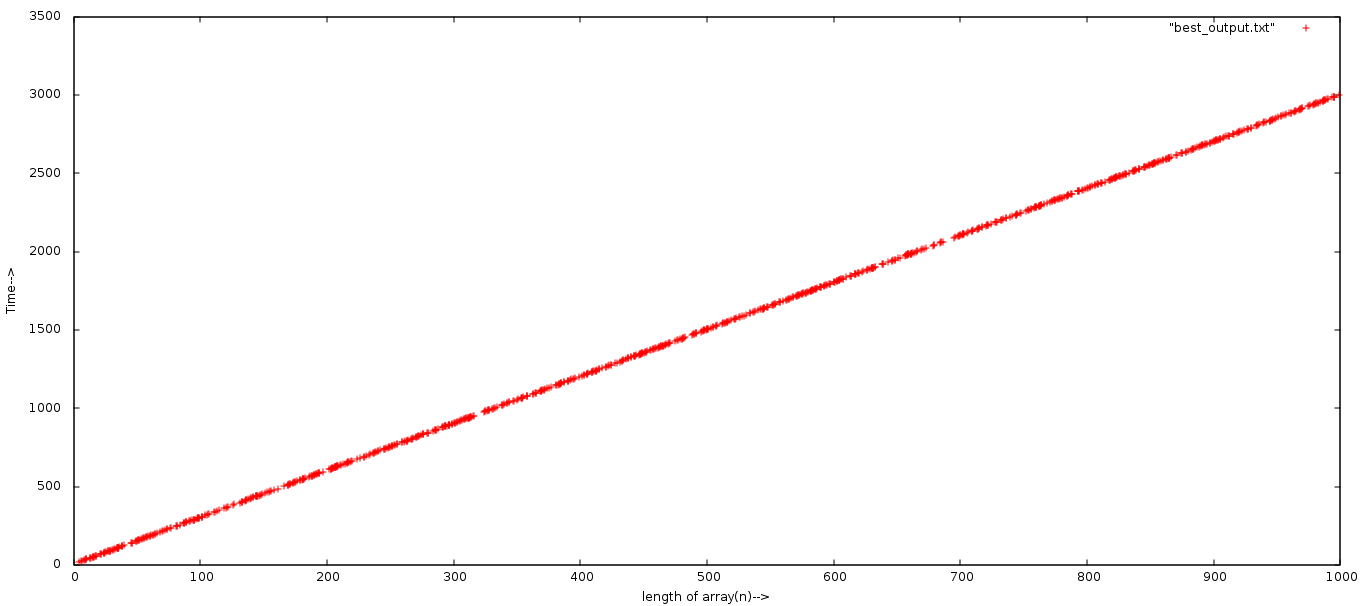
\includegraphics[height =  6.00cm,width = \linewidth]{best.png}
\textbf{Fig.1 Length of array(n) vs  Time}
\subsubsection{\textbf{Worst-Case}}
As far as worst case is concerned, we are assuming that we will place minimum element at the very beginning of array and maximum element at last. In this way, our output array should be in ascending order. By above assumption we can say that our worst case occur if the input array is in descending order. As because for worst case check will never return 1 and we will have to go into divide and conquer part.\\
For the worst case, we require the CHECK function, The  getMinMax 
function and the main function is mandatory.\\
The number of units of the time taken for the CHECK function is :- $5n+9$\\
The number of units of the time taken for the getMinMax function is :- $(3n/2)-2$ if n is power of 2
Overall time complexity of worst case is:-  $\frac{n}{2}\left(\frac{3n}{2}-2\right)$ or $O(n^2)$

 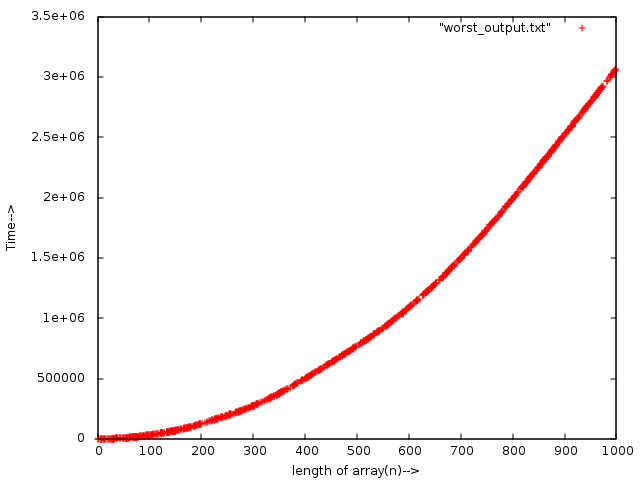
\includegraphics[height =  6.00cm,width = \linewidth]{worst.png}
 \textbf{Fig.2 Length of array(n) vs  Time}\\
\subsubsection{\textbf{Average-Case}} 
For average case we can say that it will lie between best and worst case but more accurately it is order of $n^2$ or we can say that overall time complexity for average case is $O(n^2)$.
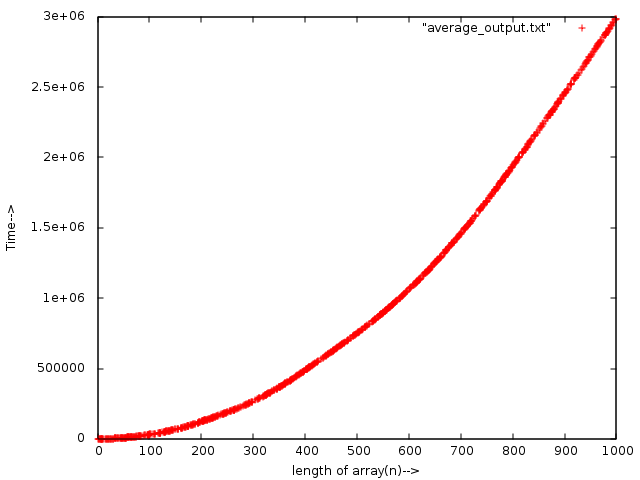
\includegraphics[height =  6.00cm,width = \linewidth]{average.png}
\textbf{Fig.3 Length of array(n) vs  Time}\\
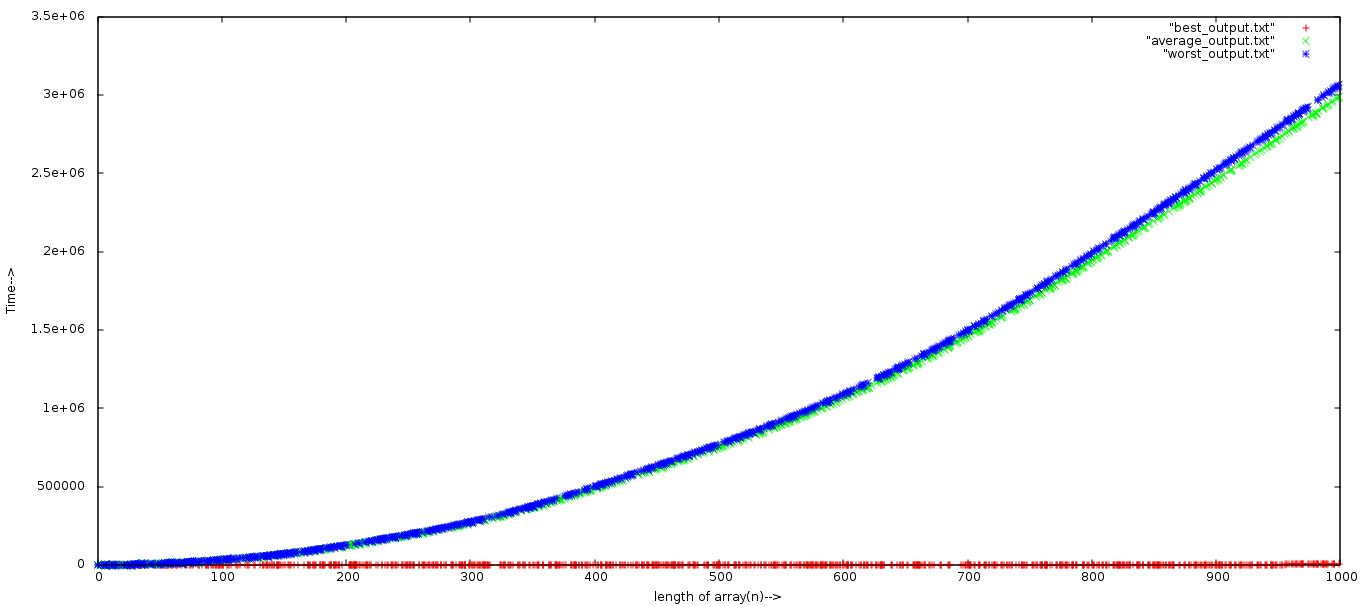
\includegraphics[height =  6.00cm,width = \linewidth]{all.png}
\textbf{Fig.4 Length of array(n) vs  Time}\\\\
RED CURVE:- \textbf{best case}\\
GREEN CURVE:- \textbf{average case}\\
BLUE CURVE:- \textbf{worst case}


\section{\textbf{Experimental Analysis}}
We revised the commands and basic functions of \textbf{GNUPlot}
to plot the time complexity analysis graphs and other relevant
analysis related to our algorithm.
\\
\	While making this report we also learnt the basics of
making reports using LATEX in IEEE format using \textbf{IEEEtran class}.
\\\\
For the analysis of the Complexity of the algorithm we had to generate 3 kinds of test cases. For each of these 3 kinds our code was run on \textbf{1000} test cases of each type and The algorithm was run on these three files separately and graphs were plotted using \textbf{GNU-Plot}.The graphs have been vividly explained in the previous section. In each of these test cases the length of \textbf{array} was randomly chosen greater then 1.
\\
\\
For the \textbf{Best case}, we generated the test cases where array is in ascending order as we have assumed that we will put minimum element at first position and maximum element at the last position
\\

For the \textbf{Worst case}, we generated test cases where array is in descending order so that for every iteration of loop we will not get any part of array being ascending already.So for every iteration we will have to go into divide and conquer part.
\\

And for the \textbf{average case}, we generated test cases where array was filled with random number. So it may be possible that any point of loop we may get array in ascending order or we may never get any array in ascending order
 \\
\begin{table}[h!]
\begin{center}
    \label{tab:table1}
    \begin{tabular}{|c|c|c|c|} % <-- Alignments: 1st column left, 2nd middle and 3rd right, with vertical lines in between
    \hline
      \textbf{n} & $\textbf{{time}}_{{best case}}$ & $\textbf{{time}}_{{average case}}$ & $\textbf{{time}}_{{worst case}}$
      \\
      \hline
      5 & 20 & 143 & 148\\
      \hline
      10 & 35 & 370 & 459\\
      \hline
      20 & 65 & 1477 & 1523\\
      \hline
      50 & 155 & 8371 & 8547\\
      \hline
	  75 & 230 & 17707 & 18063\\
      \hline
	  100 & 305 & 31745 & 32551\\
      \hline
    \end{tabular}
\end{center}
\end{table}
\\

\section{\textbf{Conclusion}}
In the problem we had to sort a given array by continuously tracking the Maximum and Minimum elements at every recursive step and placing the Maximum and Minimum elements at the correct position. We had to find the Maximum and Minimum elements by the Divide and Conquer approach. For this we used \textbf{Check function} which returns 1 if the array is in ascending order else 0. This is used to check if the array is sorted properly or not. Then the \textbf{getMinMax function} is the one where we find the Minimum and Maximum positions of the array by the Divide and Conquer approach. The best case time complexity of the problem is $O(n)$. The worst case time complexity is $O(n^2)$.And accordingly for the average case it is lying in between the best and worst case but through out the experimental analysis it is basically quite nearer to the curve for worst case.Overall the solution is optimized by the Divide and Conquer approach and it is used to calculate the Minimum and Maximum.As well as according to our convention we are sorting the input array in ascending order. 

\begin{thebibliography}{1}
\bibitem{IEEEhowto:kopka}
Introduction To Algorithms (Second Edition) by Thomas H.Cormen,
Charles E.Leiserson , R.L.Rivest and Clifford Stein.
\bibitem{}
The C Programming Language by Brian Kernighan and Dennis Ritchie.
\bibitem{}
https://www.geeksforgeeks.org/
\bibitem{}
https://www.stackoverflow.com/
\end{thebibliography}

\end{document}
